The shape of the offering formula is always the same. It opens with the same standard phrase, invokes a god to pass along the offering, lists the offerings then names the recipient.

\section*{\indexed{Htp-di-nsw}}
\markboth{Outline}{Htp-di-nsw}
\addcontentsline{toc}{section}{Htp-di-nsw}

\begin{figure} [H]
	\centering
	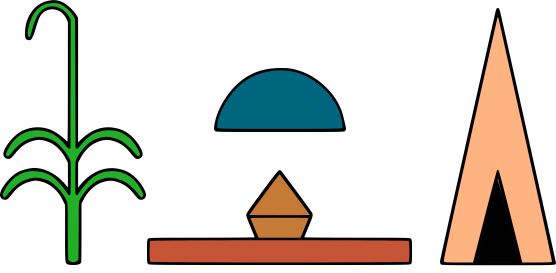
\includegraphics[width=0.4\textwidth]{../images/htp-di-nsw}
	\caption{Htp-di-nsw as commonly rendered in hieroglyphs}
\end{figure}

Many renditions of the offering formula begin with this compound expression. The exact interpretation is debated, but this is often rendered as "a royal offering" or "an offering given by the king".

This expression is sometimes used to describe an offering formula.

By convention the t from \indexed{nswt} is dropped, although it often appears in writing and inscriptions.

The order of the words when written is a case of \textit{\indexed{honorific transposition}}, with the \indexed{nswt} part written first. This is to show the importance of the king, and also applies to names of gods and the word nTr which loosely translates to "god".

\subsection*{Htp}

\begin{figure} [H]
	\centering
	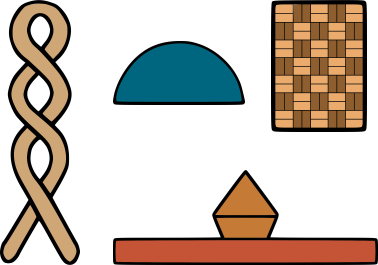
\includegraphics[width=0.275\textwidth]{../images/htp}
	\caption{A more complete spelling of \indexed{Htp} - \textbf{H t p} [Htp]}
\end{figure}

The word \indexed{Htp} has no precise translation into English, and is variously rendered as "contentment", "peace" or "offering". This is sufficient to grasp its true meaning, since offerings are intended to bring comfort and bliss.

\begin{figure} [H]
	\centering
	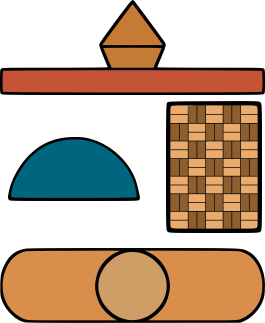
\includegraphics[width=0.175\textwidth]{../images/htp2}
	\caption{Another spelling of \indexed{Htp} - \textbf{Htp} t p [X4]}
\end{figure}

\subsection*{di}

\begin{figure} [H]
	\centering
	\includegraphics[width=0.125\textwidth]{../recoloured-tuxscribe-hieroglyphs/png/X8}
	\caption{the (r)di hieroglyph - X8}
\end{figure}

This word is a verb, (r)\indexed{di} - to give, which in older writings is sometimes rendered as \indexed{rdi} rather than di. It also appears later in the formula, but with a suffix pronoun, either .f, .s or .sn depending on the god(s) invoked.

\begin{figure} [H]
	\centering
	\includegraphics[width=0.375\textwidth]{../recoloured-tuxscribe-hieroglyphs/png/D37}
	\caption{the (r)di hieroglyph commonly used when writing di.f - D37}
\end{figure}

\subsection*{nswt}

The term nswt means the king or ruler. It was treated with great reverence as the embodiment of the institution of statehood, which was unique in its earliest form.

In older Egyptological works it is transliterated as swtn, but it is now believed that the order of the hieroglyphs is a form of \indexed{honorific transposition}.

\section*{di.f prt-xrw}
\markboth{Outline}{di.f prt-xrw}
\addcontentsline{toc}{section}{di.f prt-xrw}

\begin{figure} [H]
	\centering
	\includegraphics[width=0.25\textwidth]{../recoloured-tuxscribe-hieroglyphs/png/O3}
	\caption{the prt-xrw hieroglyph - O3}
\end{figure}

The expression \indexed{prt-xrw} is usually translated as "\indexed{voice offering}", although it more directly means "emerging from voice".

The hieroglyph contains the bread and beer signs, but this is by convention, and doesn't necessarily mean that the voice offering includes bread and beer.

It is usually preceded by the phrase di.f for a single male god passing the offering along, although there are variations for a single female god and a group of gods: di.s and di.sn.

\begin{figure} [H]
	\centering
	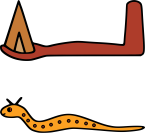
\includegraphics[width=0.125\textwidth]{../images/di-f}
	\hspace{0.1\textwidth}
	
\includegraphics[width=0.125\textwidth]{../images/di-s}
	\hspace{0.1\textwidth}
	
\includegraphics[width=0.169643\textwidth]{../images/di-sn}
	\caption{Standard spellings of \textbf{di}.\textbf{f}, \textbf{di}.\textbf{s} and \textbf{di}.\textbf{sn}}
\end{figure}

\section*{Offering(s)}
\markboth{Outline}{Offerings}
\addcontentsline{toc}{section}{Offerings}

\begin{figure} [H]
	\centering
	
\includegraphics[width=0.875\textwidth]{../images/xt-nb-nfr-wab-anxt-ntr-im}
	\caption{\textbf{x t nb}(t) \textbf{n f r} nfr (t) \textbf{wab} (t) \textbf{anx} n x \textbf{t nTr i m}}
\end{figure}

Thee is something of a standard list of offerings, which is usually terminated with the expression xt nbt nfrt wabt anxt nTr im - all the beautiful and pure things on which a god lives.

\subsection*{Bread - t}

\begin{figure} [H]
	\centering
	\includegraphics[width=0.2\textwidth]{../recoloured-tuxscribe-hieroglyphs/png/X1}
	\caption{the t hieroglyph - X1}
\end{figure}

Bread\index{bread} was a staple in the diet of Ancient Egypt, and bread making and consumption was deeply integrated into their culture.

It was primarily made from emmer \indexed{wheat} or \indexed{barley}, which was ground into \indexed{flour} using stones. The dough, made by mixing with \indexed{water}, and sometimes \indexed{honey} or \indexed{oil}, was left to naturally ferment, giving it a slightly sour flavour. Baking was usually done in conical \indexed{clay} \indexed{oven}s, where the dough was either placed on the oven walls, or baked in molds.

The hieroglyph for (r)di, X8, represents a sacrificial loaf, although it is a highly stylised rendition. The hieroglyph for t, X1, is also a stylised loaf. In the prt-xrw hieroglyph we can see X3 also used to represent a loaf.

\begin{figure} [H]
	\centering
	\includegraphics[width=0.125\textwidth]{../recoloured-tuxscribe-hieroglyphs/png/X3}
	\caption{the bread hieroglyph - X3}
\end{figure}

\subsection*{Beer - Hnqt}

Beer\index{beer} was an integral part of daily life in ancient Egypt, enjoyed by both the rich and the poor. Famously it was used to pay workers on the great royal projects, including the construction of the \indexed{Great Pyramid} of \sname{Giza}.

\begin{figure} [H]
	\centering
	\includegraphics[width=0.125\textwidth]{../recoloured-tuxscribe-hieroglyphs/png/W22}
	\caption{the Hnqt hieroglyph - W22}
\end{figure}

It was primarily made from the aforementioned \indexed{bread}, which was crumbled into \indexed{water} and left to ferment. The resulting brew was thick and nutritious, often flavoured with herbs, \indexed{honey}, or \indexed{fruit}s.

\subsection*{Oxen - kAw}

\begin{figure} [H]
	\centering
	\includegraphics[width=0.25\textwidth]{../recoloured-tuxscribe-hieroglyphs/png/F1}
	\caption{the kA(w) hieroglyph - F1}
\end{figure}

In ancient Egypt, \indexed{oxen}, castrated \indexed{bull}s, were highly valued for their critical role in agriculture and daily life. These sturdy animals were used for plowing fields, threshing grain, and transporting heavy loads, making them indispensable for farming communities along the \sname{Nile}.

Bulls\index{bull} and \indexed{cow}s themselves were often part of religious ceremonies and offerings, representing strength and fertility. The \indexed{cow} was sacred to \nname{Hathor}, and certain sacred bulls were considered as gods themselves, including the \nname{Apis}, \nname{Mnevis} and \nname{Buchis} bulls.

Beef seems to have been considered somewhat of a luxury and was typically reserved for the elite and for special occasions.

Tomb paintings and carvings frequently depicted scenes of cattle being tended to, highlighting their importance in both practical and ceremonial contexts.

\subsection*{Fowl - Apdw}

\begin{figure} [H]
	\centering
	\includegraphics[width=0.2\textwidth]{../recoloured-tuxscribe-hieroglyphs/png/H1}
	\caption{the Apd(w) hieroglyph - H1}
\end{figure}

In ancient Egypt, \indexed{fowl} such as \indexed{duck}s, geese\index{goose}, pigeons, and quails played a significant role in both daily life and religious practices. In particular pigeons were trained as carriers for communication.

These birds were commonly raised in households and on farms, as well as being harvested from the river itself. They provided a source of meat, eggs, and feathers.

The Egyptians employed various techniques to catch wild birds, including netting and trapping. Fowl were often depicted in tomb paintings and reliefs, showcasing their importance in the Egyptian diet and culture.

\subsection*{Alabaster - Ss}

\begin{figure} [H]
	\centering
	\includegraphics[width=0.125\textwidth]{../recoloured-tuxscribe-hieroglyphs/png/V6}
	\caption{the Ss hieroglyph - V6}
\end{figure}

Alabaster, more specifically \indexed{calcite} \indexed{alabaster} or \indexed{travertine}, is a type of finely-grained translucent \indexed{stone}. It was highly prized in ancient Egypt for its beauty and versatility. This soft, workable material was especially favoured for sculpting intricate \indexed{statue}s, jars, and ceremonial vessels due to its smooth surface and ability to be carved with great precision. It was also employed in the production of \indexed{canopic jar}s that held the organs of the deceased during mummification.

\subsection*{Linen - mnxt}

\begin{figure} [H]
	\centering
	\includegraphics[width=0.25\textwidth]{../recoloured-tuxscribe-hieroglyphs/png/S27}
	\caption{the mnxt hieroglyph - S27}
\end{figure}

Linen was one of the most important textiles in ancient Egypt, renowned for its lightweight, breathable properties, and high quality.

Made from the fibres of flax plants, linen was used to produce a wide range of items, including clothing, bedsheets, and wrappings for mummies. The process of making linen involved harvesting flax, soaking it to loosen the fibres, and then spinning and weaving those fibres into fabric.

Finished linen ranged from coarse to fine, with the finest quality reserved for the elite and for religious and ceremonial purposes. It would be naturally bleached in the sun to create the fine white linens we see worn in tomb paintings.

It is fairly common to see alabaster and linen in offering formulae using a combined hieroglyph.

\begin{figure} [H]
	\centering
	\includegraphics[width=0.25\textwidth]{../recoloured-tuxscribe-hieroglyphs/png/S113}
	\caption{the Ss-mnxt hieroglyph - S113}
\end{figure}

\section*{God(s)}
\markboth{Outline}{God(s)}
\addcontentsline{toc}{section}{God(s)}

\subsection*{Anubis, who sits on his mountain}
\addcontentsline{toc}{subsection}{Anubis, who sits on his mountain}

\begin{figure} [H]
	\centering
	\includegraphics[width=0.0625\textwidth]{../recoloured-tuxscribe-hieroglyphs/png/C6}
	\hspace{0.03125\textwidth}
	\includegraphics[width=0.125\textwidth]{../recoloured-tuxscribe-hieroglyphs/png/E16}
	\includegraphics[width=0.125\textwidth]{../recoloured-tuxscribe-hieroglyphs/png/E17}
	\includegraphics[width=0.125\textwidth]{../recoloured-tuxscribe-hieroglyphs/png/E18}
	\caption{Single hieroglyphs for inpw - C6, E16, E17 and E18}
\end{figure}

Anubis is one of ancient Egypt's most revered and enigmatic deities. He is widely recognized as the god of mummification and the protector of the dead. He was often invoked in offering formulae, especially the oldest examples we have from the \indexed{Old Kingdom}.

\begin{figure} [H]
	\centering
	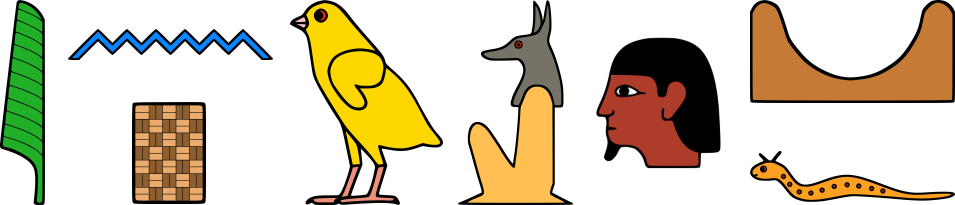
\includegraphics[width=0.875\textwidth]{../images/inpw-tpy-dwf}
	\caption{Anubis, who sits on his mountain\\\textbf{i n p w} [inpw] \textbf{tp} (y) \textbf{Dw.f}}
\end{figure}

Often depicted as a man with the head of a \indexed{jackal}, or entirely as a jackal, Anubis embodies the dual aspects of fear and reverence that surrounded death and the afterlife in ancient Egyptian culture.

\begin{figure} [H]
	\centering
	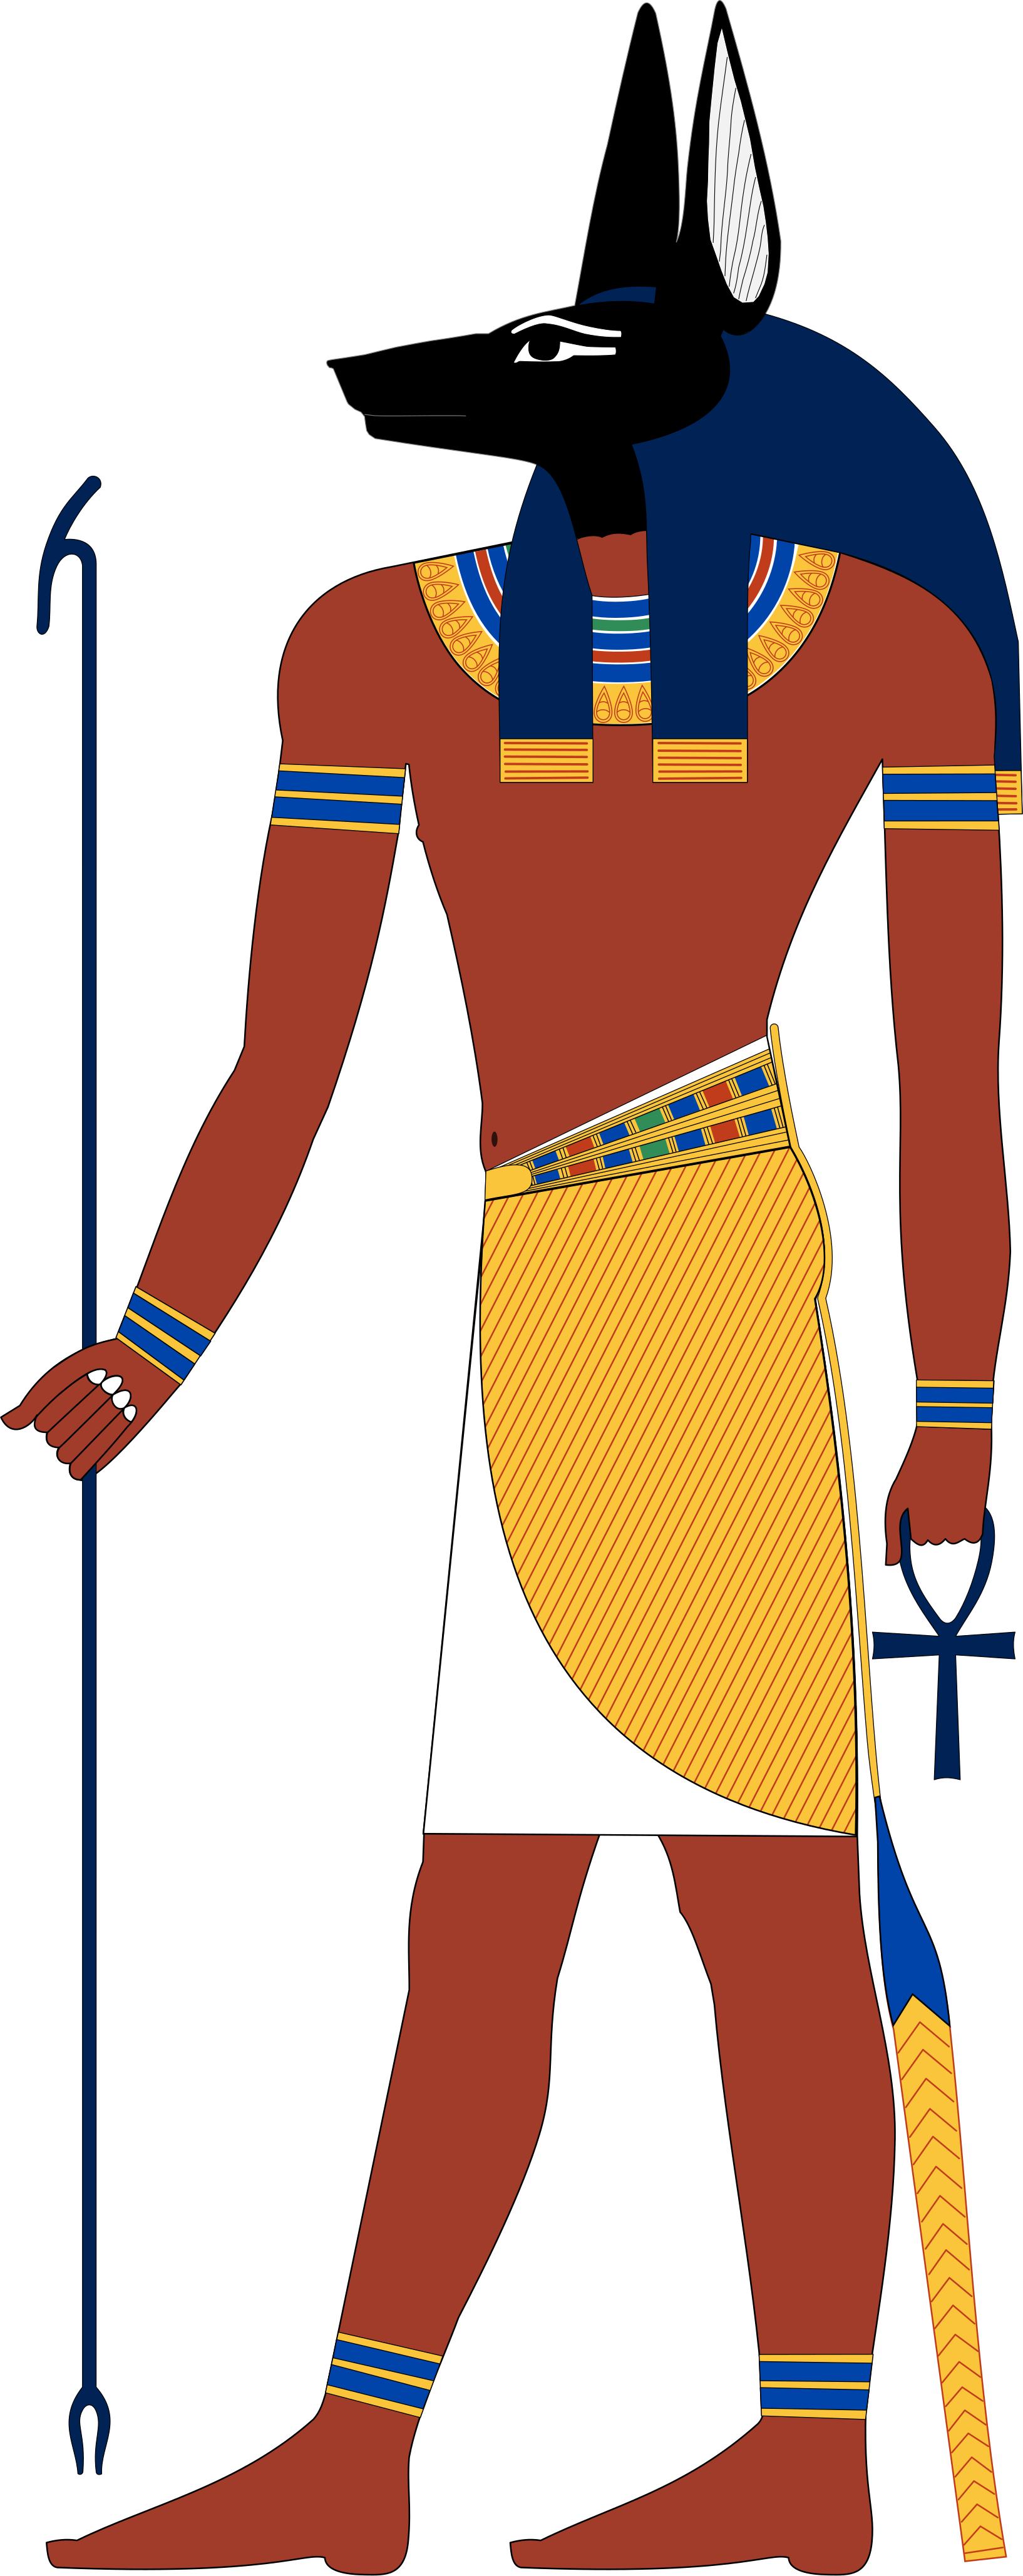
\includegraphics[width=0.5\textwidth]{../images/anubis}
	\caption{A standard depiction of Anubis holding the ankh and a was sceptre}
\end{figure}

\subsubsection*{Origins and myths}
\addcontentsline{toc}{subsubsection}{Origins and myths}
The worship of \nname{Anubis} goes back to the predynastic period of Egyptian history.

His association with the \indexed{jackal} - a creature commonly seen around cemeteries and tombs - emphasize his role as a guardian of the necropolis, where the dead were laid to rest.

Initially, he was considered the foremost deity of the dead, a role later overshadowed by Osiris. However, \nname{Anubis} retained significant influence as the embalmer and guide of souls. Myths recount his critical role in the legend of \nname{Osiris} - he embalmed \nname{Osiris} after his murder by \nname{Seth}, making him the first \indexed{mummy} and setting the standards for \indexed{embalming} rites.

\subsubsection*{Iconography and symbols}
\addcontentsline{toc}{subsubsection}{Iconography and symbols}

The iconography of \nname{Anubis} is striking and distinctive. He is frequently depicted as a jackal, in a crouching or alert position, sometimes vigilant at the entrance of a tomb. His sleek black body has the colour associated with embalming, rebirth and the fertile soil of the \sname{Nile} inundation.

\begin{figure} [H]
	\centering
	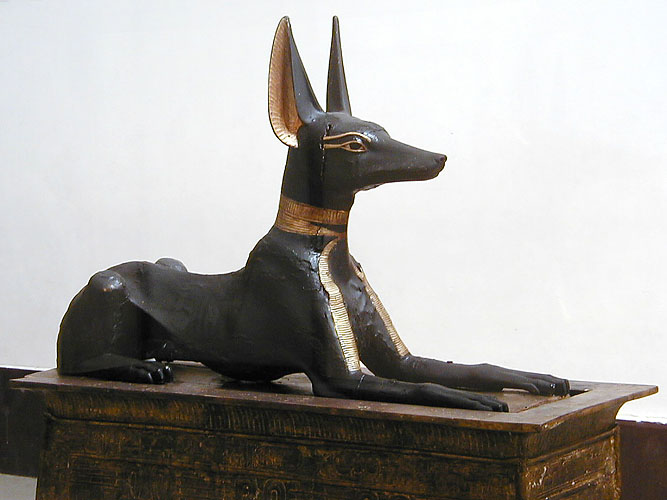
\includegraphics[width=0.75\textwidth]{../photos/Tutankhamun_Jackal}
	\caption{A guardian jackal statue from the tomb of Tutankhamun\\(Photo by Jon Bodsworth)}
\end{figure}

\nname{Anubis} was commonly depicted in the \indexed{weighing of the heart} ceremony - weighing the hearts of the deceased against the feather of \nname{Ma'at}, the goddess of truth and justice, in the Hall of two Ma'ats. This ceremony determined whether the deceased could continue in the journey to the afterlife.

\begin{figure} [H]
	\centering
	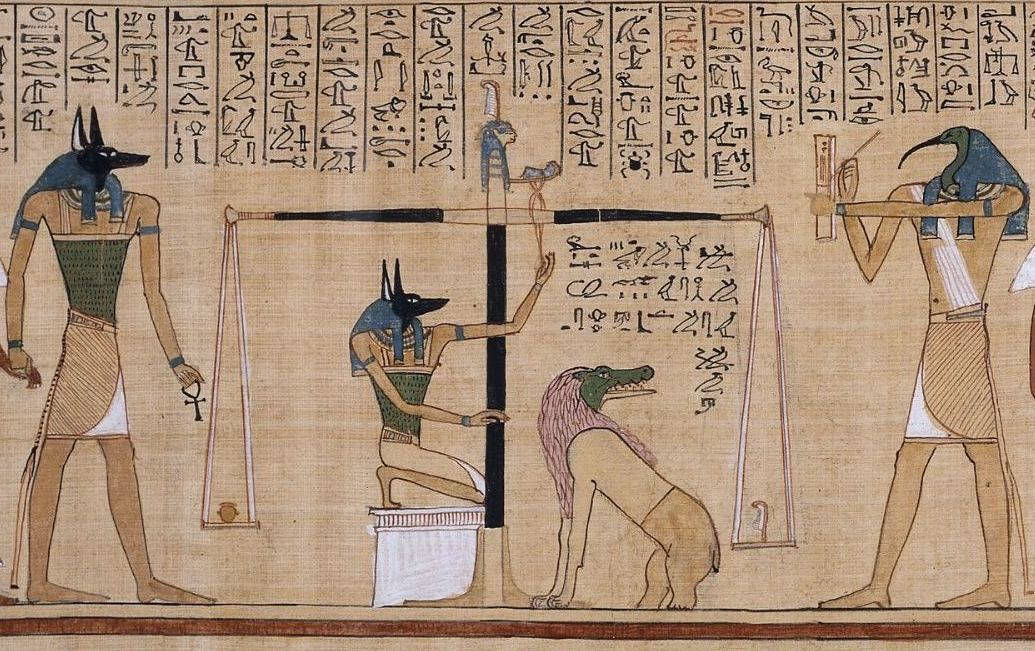
\includegraphics[width=0.75\textwidth]{../photos/Anubis_Hunefer}
	\caption{The weighing of the heart from the \indexed{Book of the Dead} of Hunefer}
\end{figure}

In another common representation, \nname{Anubis} is shown attending to a mummy, highlighting his role in embalming.

\begin{figure} [H]
	\centering
	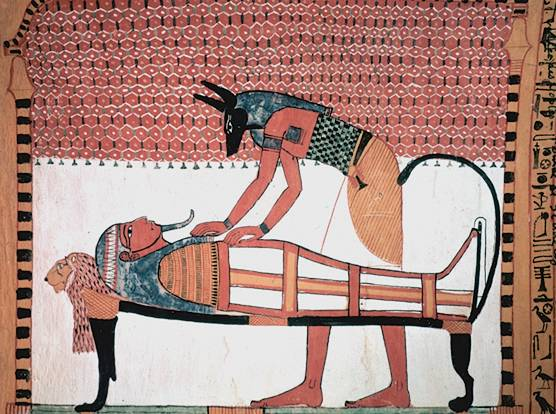
\includegraphics[width=0.75\textwidth]{../photos/Anubis_Sennedjem}
	\caption{Anubis, depicted attending the mummy of Sennedjem}
\end{figure}

His primary symbols include the \indexed{flail} reflecting his purifying role in selecting those deserving of the afterlife, and the \indexed{imy-wt}, or "\indexed{Anubis fetish}" - a stuffed, headless animal skin supported by a rod. In addition he is often depicted with the symbols of godhood, the \indexed{ankh}, a symbol of life and the \indexed{wAs} sceptre, signifying his authority.

\subsubsection*{Epithets}

TODO: ... epithets

\subsubsection*{Cult and worship}
\addcontentsline{toc}{subsubsection}{Cult and worship}
The worship of \nname{Anubis} was pervasive throughout Egypt, but there was a significant cult centre at sAkA, known by the \indexed{Greek}s as \sname{Cynopolis} (city of the dog). Priests of \nname{Anubis} were tasked with overseeing mummification and funerary rites, donning jackal masks during ceremonies to invoke his presence. Rituals performed in his honour aimed to ensure the safe passage of the dead into the afterlife, with particular emphasis on purity and protection.

Amulets bearing the likeness of Anubis or his symbols were commonly placed among the burial goods, intended to ward off malevolent forces and guide the deceased through the treacherous journey to the afterlife. These artefacts, often inscribed with spells from the \indexed{Book of the Dead}, reflect strong belief in the ability of \nname{Anubis} to safeguard and guide the deceased.

\subsubsection*{Legacy}
The legacy of \nname{Anubis} endured well beyond the end of the pharaonic era. His image and role were integrated into Greco-Roman culture, where he was often syncretized with \nname{Hermes}, or forming the composite god \nname{Hermanubis}, embodying both \indexed{Greek} and Egyptian aspects of the afterlife.

In modern times, \nname{Anubis} remains a potent symbol in popular culture, representing the ancient Egyptian fascination with death and the afterlife. He appears in literature, films, and other media, continuing to captivate imaginations with his mysterious and powerful presence.

The enduring legacy of \nname{Anubis} underscores the ancient Egyptians' profound respect for the dead and their meticulous rituals to ensure safe passage into the afterlife. As the eternal guardian of the necropolis, Anubis epitomizes the delicate balance between life, death, and the promise of rebirth - a timeless reflection of humanity's quest for understanding the mysteries that lie beyond.

\subsection*{Osiris, lord of Abydos}
\addcontentsline{toc}{subsection}{Osiris, lord of Abydos}

\nname{Osiris} stands as one of the most prominent and beloved gods in ancient Egyptian mythology, representing resurrection, the \indexed{afterlife}, and eternal \indexed{king}ship. Revered as the god of the dead, the story of \nname{Osiris} is both a tale of tragedy as well as triumph, reflecting ancient Egyptian beliefs about \indexed{death} and \indexed{rebirth}.

\begin{figure} [H]
	\centering
	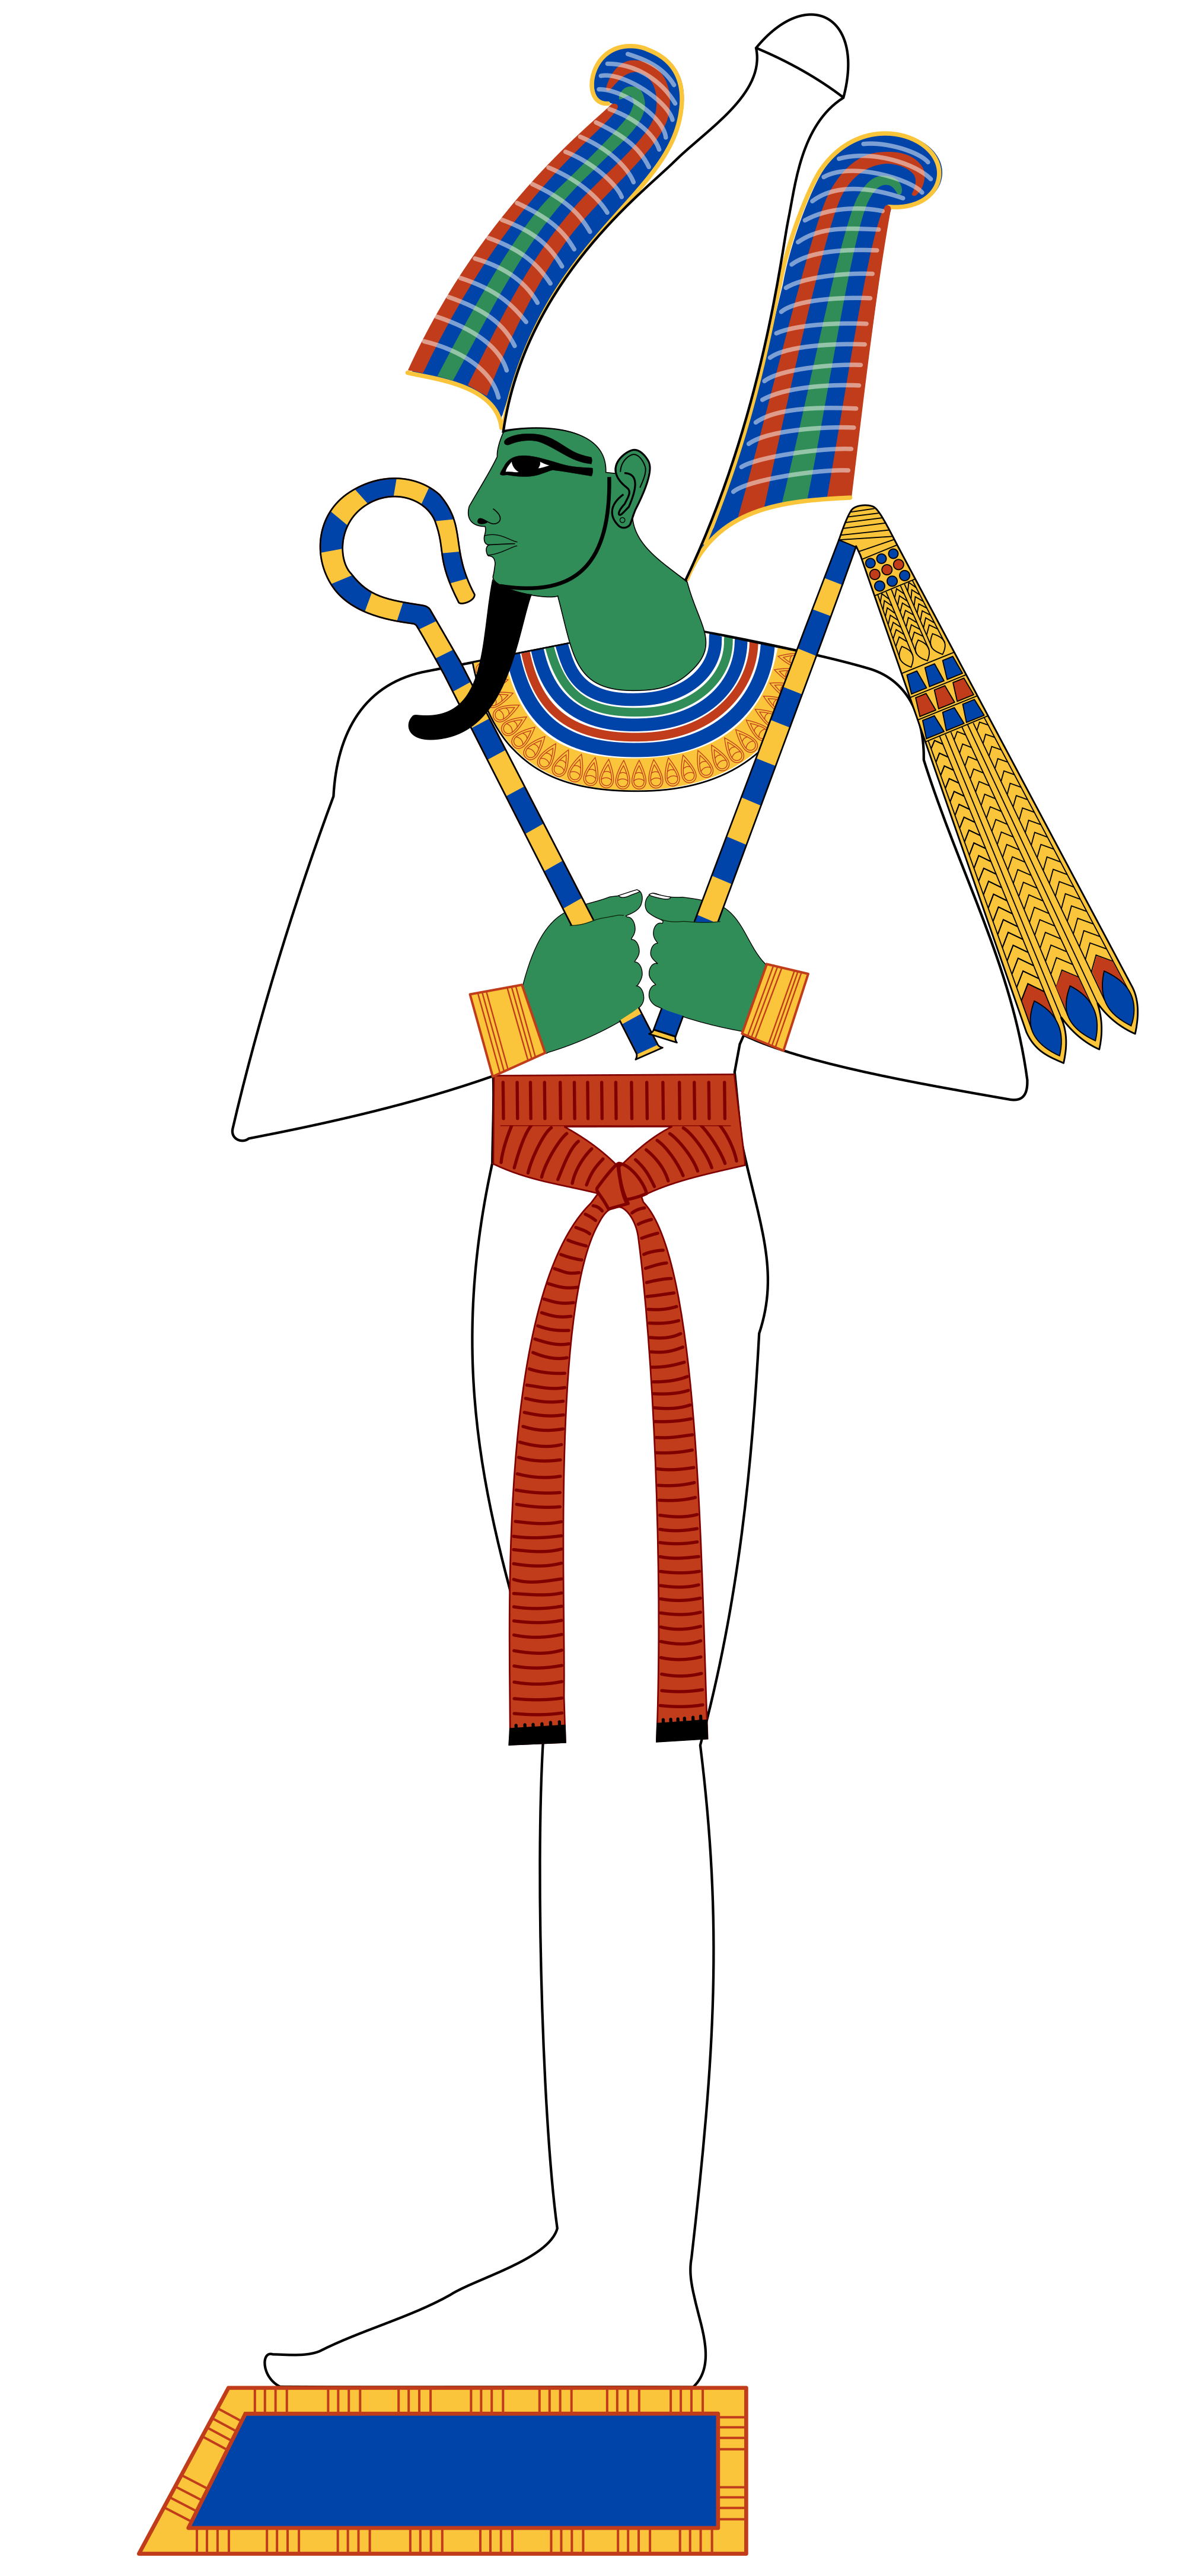
\includegraphics[width=0.5\textwidth]{../images/osiris}
	\caption{A standard depiction of \nname{Osiris} as a mummy wearing the \indexed{atef} \indexed{crown}, and holding the \indexed{crook} and \indexed{flail}}
\end{figure}

\subsubsection*{Origins and myths}

\nname{Osiris} is the subject of, perhaps, the most famous of all ancient Egyptian myths.

\nname{Osiris} was the eldest son of the earth god \nname{Geb} and the sky goddess \nname{Nut}, making him a central figure in the divine pantheon. He was married to his sister \nname{Isis}, forming a powerful and revered couple. \nname{Osiris} was initially a great \indexed{king} of \sname{Egypt}, ruling wisely and bringing civilization to his people. However, his reign was cut short by betrayal and murder at the hands of his jealous brother \nname{Seth}, who sought to usurp the throne.

There are many variations of the myth, but something like a standard version is given here.

\nname{Seth} tricked \nname{Osiris} into becoming trapped in a coffin and cast it into the \sname{Nile}, where it eventually crossed the \indexed{Mediterranean} (\indexed{wAD-wr}) and came to rest in the land of \sname{Byblos}. \nname{Isis}, heartbroken and determined, set out to find her husband's body. With the help of her sister \nname{Nephthys}, she discovered the coffin and brought it back to \sname{Egypt}.

However, \nname{Seth} found the body again and dismembered it into 42 pieces, scattering them across the land, one for each \indexed{nome} of \sname{Egypt}. Undeterred, \nname{Isis}, \nname{Nephthys}, and \nname{Anubis} meticulously gathered the pieces, reassembled \nname{Osiris}, and wrapped him in linen, creating the first \indexed{mummy}. Through her magical abilities, \nname{Isis} breathed life back into \nname{Osiris}, allowing him to become the ruler of the \indexed{afterlife}.

\subsubsection*{Iconography and symbols}

\nname{Osiris} is typically depicted as a mummified king, with green or black skin symbolizing fertility, regeneration, and the rich life giving silt from the inundation of the \sname{Nile}. He is often shown wearing the \indexed{atef} crown, a white crown flanked by two \indexed{ostrich} feathers, and holding the \indexed{crook} and \indexed{flail} — emblems of kingship and authority. His images evoke the promise of rebirth and the eternal cycle of life and death.

\begin{figure} [H]
	\centering
	\includegraphics[width=0.0625\textwidth]{../recoloured-tuxscribe-hieroglyphs/png/S38}
	\caption{the crook - HqA hieroglyph - S38}
\end{figure}

A central symbol associated with \nname{Osiris} is the "\indexed{djed} pillar," representing stability and endurance. This iconic symbol, often seen in temple reliefs and funerary texts, signifies the role of \nname{Osiris} as a source of strength and renewal. The \indexed{djed} (Dd) pillar is also used in rituals and festivals dedicated to \nname{Osiris}, such as the annual "Raising of the Djed" ceremony, which symbolizes his resurrection.

\begin{figure} [H]
	\centering
	\includegraphics[width=0.0625\textwidth]{../recoloured-tuxscribe-hieroglyphs/png/R11}
	\caption{the Dd hieroglyph - R11}
\end{figure}

\subsubsection*{Epithets}

TODO: ... epithets

\subsubsection*{Cult and worship}

The cult of Osiris was widespread throughout ancient Egypt, with significant centers of worship in \sname{Abydos} (AbDw), where his tomb was believed to be located, and in \sname{Busiris} (Ddw), in the \sname{Nile} \sname{Delta}. \sname{Abydos}, in particular, became a major pilgrimage site, where \indexed{festival}s and processions reenacted Osiris's death and resurrection. Devotees participated in these \indexed{ritual}s to ensure their own safe passage to the \indexed{afterlife} and to receive blessings from \nname{Osiris}.

The role of \nname{Osiris} as the judge of the dead is well-documented in ancient Egyptian religious texts, including the \indexed{Book of the Dead}. In the Hall of Two \nname{Ma'at}s, \nname{Osiris} presides over the weighing of the heart ceremony.

\subsubsection*{Legacy}

The legacy of \nname{Osiris} endures not only in ancient Egyptian religion but also in the broader context of global mythology and spirituality. His story of \indexed{death} and \indexed{rebirth} has parallels in other cultures and religions, symbolizing the universal themes of transformation and growth. In Greco-Roman times, \nname{Osiris} was often associated with \nname{Dionysus} and other deities of the \indexed{afterlife}, reflecting the cross-cultural exchange of ideas and beliefs.

In modern times, \nname{Osiris} continues to capture the imagination of scholars, artists, and the general public. His story is retold in literature, films, and various forms of media, highlighting the enduring fascination with his myth and the profound impact of ancient Egyptian culture on the world.

\subsection*{Hathor, lady of the west}
\addcontentsline{toc}{subsection}{Hathor, lady of the west}

\begin{figure} [H]
	\centering
	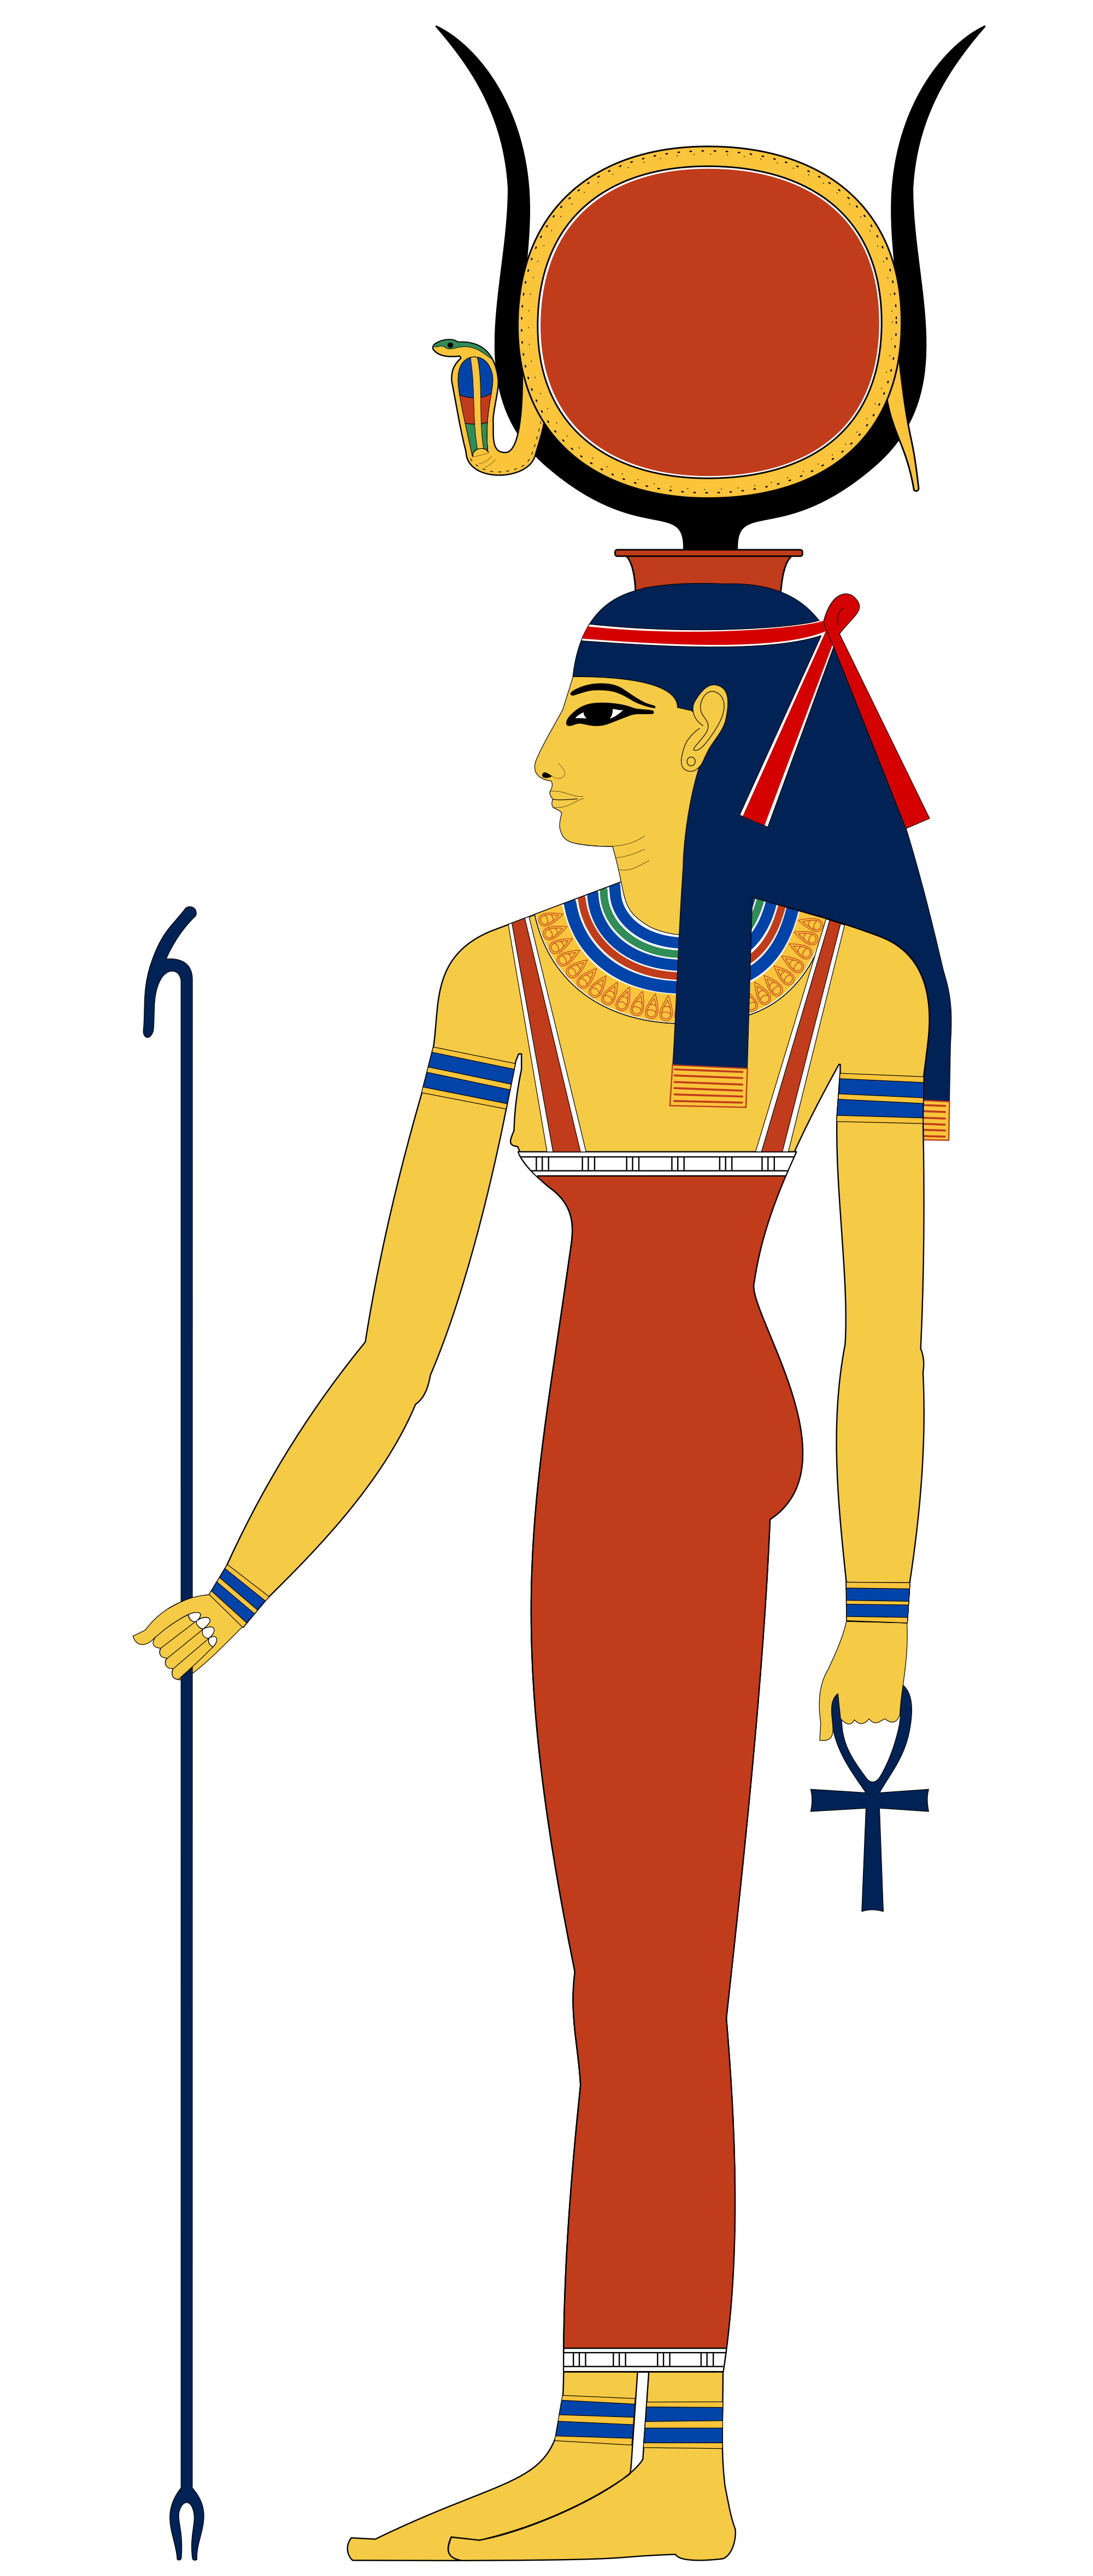
\includegraphics[width=0.5\textwidth]{../images/hathor}
	\caption{A standard depiction of \nname{Hathor}}
\end{figure}

\nname{Hathor}'s influence permeated many aspects of daily life and religious practice in ancient \sname{Egypt}. Her nurturing and protective qualities made her a favoured goddess amongst Egyptians, from the humble commoner to the mightiest of \indexed{pharaoh}s.

\nname{Hathor}, was one of the most versatile and beloved deities in ancient Egyptian mythology, as a goddess of \indexed{love}, \indexed{music}, \indexed{dance}, \indexed{mother}hood, and \indexed{joy}. She was, however, often referred to as the lady of the \indexed{west}, reflecting her role as a \indexed{psychopomp}.

\subsubsection*{Origins and myths}

According to myth, \nname{Hathor} was born from the eye of \nname{Ra}, the \indexed{sun} god, and over time she absorbed aspects of the sky goddess \nname{Nut}.

Her name, Hwt-Hr means something like "House of \nname{Horus}", although the Hwt hieroglyph is also used for temples and other enclosures. This relates to her role as a \indexed{sky} goddess, but perhaps also as a wife of \nname{Horus}.

\subsubsection*{Iconography and symbols}

\nname{Hathor} was sometimes depicted as a cow, symbolizing fertility and abundance, or as a woman with cow horns and a solar disk on her head, signifying her connection to the sun.

\subsubsection*{Epithets}

TODO: ... epithets

\subsubsection*{Cult and worship}

Temples dedicated to \nname{Hathor} were scattered across Egypt, each a testament to her widespread veneration. The most famous of these is perhaps the temple at Dendera, a magnificent structure adorned with intricate carvings and hieroglyphs. Here, priests and priestesses performed daily rituals to honour \nname{Hathor}, including music, dance, and offerings of food and drink.

Festivals in \nname{Hathor}'s honour were grand events usually inteneded as joyous celebrations. The \indexed{Festival of Drunkenness}, for example, commemorated \nname{Hathor}'s role in saving humanity from destruction by the sun god's wrath. Legend has it that she pacified Ra by consuming red beer, which she mistook for blood, and in her intoxication, she became a force of benevolent protection.

\subsubsection*{Legacy}

The legacy of \nname{Hathor} endures in the rich tapestry of Egyptian mythology and art. Her image, often adorned with symbols of fertility and celestial power, continues to captivate and inspire. \nname{Hathor}'s story is one of love, protection, and joyous celebration, reflecting the enduring human connection to the divine.

\section*{n kA n}

The offering formula is directed at the \indexed{kA} of the recipient.

\section*{mAa-xrw}

True of voice.

\section*{Putting it all together}